\documentclass[dvips,dvipdfm,pdftex]{llncs}
\usepackage[utf8]{inputenc}
\usepackage{amsmath}
\usepackage{amsfonts}
\usepackage{amssymb}
\usepackage[dvips,dvipdfm,pdftex]{graphicx}
\usepackage{pgfplotstable}
\usepackage{array}
\usepackage{booktabs}
\usepackage{morefloats}
\usepackage{etex}
\usepackage{listings}
\usepackage{float}

\title{Semi-supervised Hidden Markov Random Fields (HMRF) Kmeans. Theory to Implementation\\}
\author{Dimitrios Pritsos and Efstathios Stamatatos}
\institute{University of the Aegean\\Karlovassi, Samos \textendash{} 83200, Greece.\\\{dpritsos, stamatatos\}@aegean.gr }

\begin{document}

\maketitle

\begin{abstrat}

\end{abstrat}


\section{Introduction}\label{sec:intro}
The objective of the Semi-supervised Clustering is to incorporate in the procedure of clusters discovery or assignment, the prior knowledge about the skeleton of the clusters schema. There are several efforts on Semi-supervised model inference in both Expectation Maximization (EM) clustering based models and in Agglomerating clustering based models. According to \cite{chapelle2006semi_hmrf_kmeans} there three main groups of EM based semi-supervised clustering methods:

\begin{enumerate}
	\item \emph{Constraints-based mehtods} are using the provided supervision for guiding the algorithm towards a data partitioning which is avoiding (but not prevening) the constraints violation.
	\item \emph{Distance-based approaches} in clustering method with a particular distance funciton; the distance function is parametrized and the parameters values are learned to satisfy the constraints.
	\item \emph{Semi-supervised clustering based on Hidden Markov Random Fields} where the constraint-based and distance-based approaches are combined into \emph{a unified probabilistic model}.
\end{enumerate}

In EM clustering based models there have been several efforts where the labeled data where provided in the clustering model in the form of data-labels pairs or in the initialization phase of theclustering model. In this work we present the Hidden Markov Random Fields Model(HMRF) Kmeans, where the prior knowledge about the structure or skeleton of the clusters schema has been embedded into the model in the form of constraints \cite{basu2004probabilistic}. The HMRF Kmeans is a hard-clustering model due to the \emph{hard} assignment of the data point to one of the a-priori fixednumber of clusters. However, the same models can be transformed into a relatively easy soft-clustering model where of each data point only Maximum a-posteriry Probability (MAP) of the point to bea member of each cluster of th final schema.

The HMRF Kmeans Semi-supervised clustering method it has been implemented, in this work, for being tested on the Web Genre Identification (WGI) Information Retrieval (IR) taxonomy problem.Therefore, here we only present the model inference procedure where the distance measure, a.k.a distortion function/measure, is the cosine similarity because in the IR literature is the distortionmeasure where in most cases maximizes performance in problems where the feature space is particularly large, as in this case. In case one would be interested in changing the model to asoft-clustering method then the probability destiny function of the final model should have been chosen to be some properly parametrized Von Mises Fisher distributions.

Since this work is focusing on the implementation of Semi-supervised HMRF-Kmeans in the IR domain framework, it has to be noted that this Semi-supervised model advantage is the interactivelearning setting where this model can be used \cite{chapelle2006semi_hmrf_kmeans}, since the constraints are provided to the model in two different sets the \emph{Must-Link} and\emph{Cannot-Link}. These sets are not necessarily the same in size or complimentary one to the other.

What it follows is the model inference line of thought based on the there resources \cite{basu2004probabilistic,chapelle2006semi_hmrf_kmeans,bishop2006_EM_general_view}.

\section{Model inference}\label{sec:model_inference}
The objective of a semi-supervised model like HMRF Kmeans is to drive the procedure of clustering schema taking into account the prior knowledge we have about the clusters in the form of\emph{must-link} and \emph{cannot-link} constraints. The main difference in the graphical model of a topical EM algorithm is the nodes of the observed labeled data over the hidden, a.k.a latent,variables as depicted in fig.\ref{fig:hmrf_em}, with red colored arrows and gray shaded nodes.

\begin{figure}[h]
	\begin{center}
		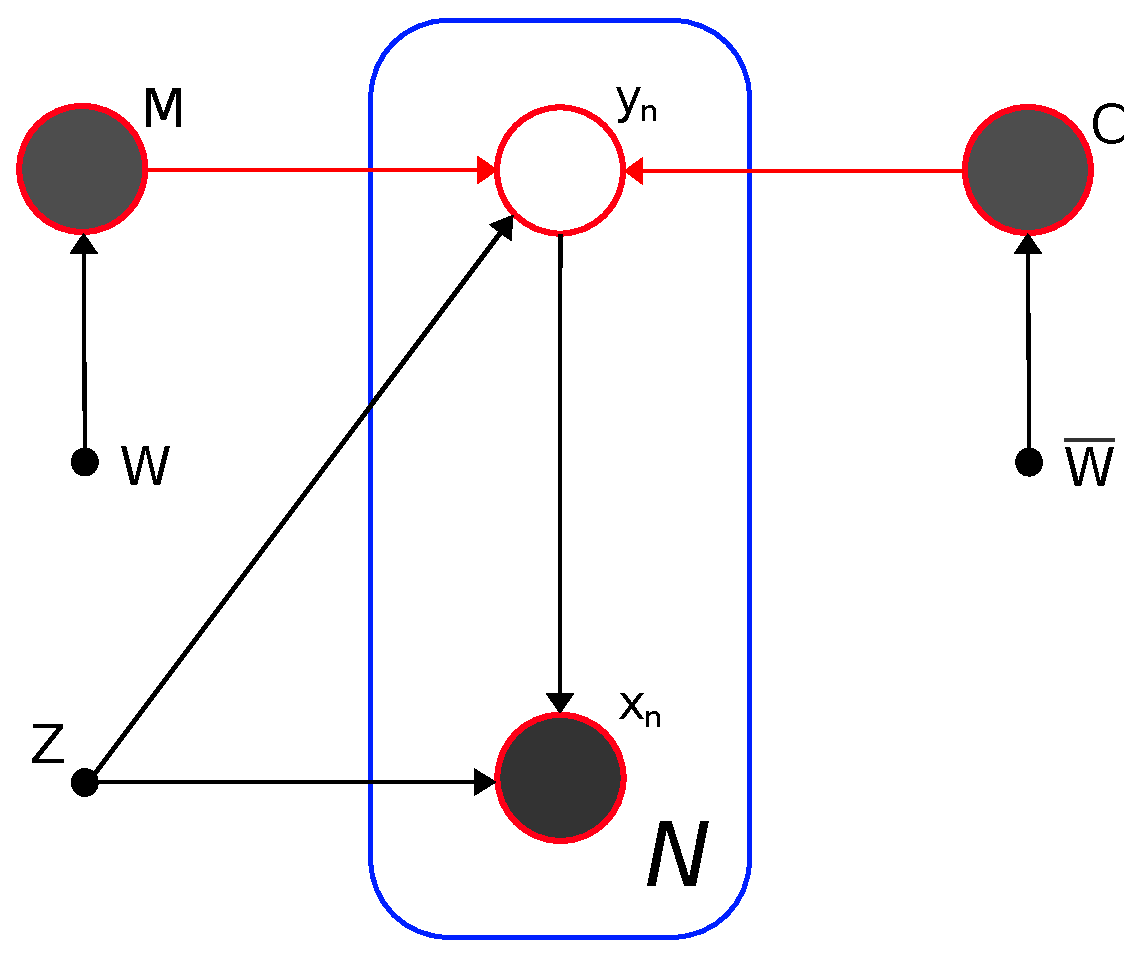
\includegraphics[scale=0.40]{figures/SemiSupervised_HMRF_EM_Graphical_Model.eps}
		\caption{Semi-supervised HMRF Expectation Maximization or Kmeans Clustering Graphical Model.}
		\label{fig:hmrf_em}
	\end{center}
\end{figure}

The goal of EM is to maximize the \emph{log likelihood function} $P(X|\Theta)$ with respect of $\Theta$ as in eq.\ref{eq:em_log_likelihood}.

\begin{equation}
lnP(X|\Theta)=ln\left\{ \sum_{l}P(X,L|\Theta)\right\}
\label{eq:em_log_likelihood}
\end{equation}

Where $X=\{\mathbf{x}_{i}\}_{i=1}^{N}$ is the set of \emph{observable random variables} given by the conditional probability $P(X|\Theta)$ and $\mathbf{x}_{i}$ is a random vector (or data point) of the corpus under taxonomy. Note the boldface notation of the random vector in order not to be mixed with $x_{i}$ which will a feature (or variable) of this vector. Moreover, $N$ is the number of vector as depicted in the graphical model of fig.\ref{fig:hmrf_em}.

Due to the relatively complex marginal distributions, like $P(X|\Theta)$, over observed data points where they are computationally intractable, there is a common practice to incorporate \emph{latent or hidden variables} in order to express the conditional probability calculation more tractable over the expanded space of observed and latent variables. In eq.\ref{eq:em_log_likelihood} $L$ is the set of hidden (or latent) variables over $X$ observable data points \cite{bishop2006_EM_general_view}.

###################### l should become a vector \mathbf{l} because can have several possible probabiliies for each of the K states (K clusters). In the hard-clustering set-up is just a value in {1,...,K}############ FIX IT IN THE WHOLE DOC

Therefor \emph{a hidden field} $L=\{l_{i}\}_{i=1}^{N}$ random variables, \emph{whose values are unobservable}. In the clustering framework, the set of hidden variables are the unobserved cluster labels on the
points, indicating cluster assignments. Every hidden variable $l_{i}$ takes values from the set ${1, . . . , N}$, which are the labels of the clusters.

Now every random data point $\mathbf{x}$ can be generated from a conditional probability distribution $P(\mathfb{x}_{i}|l_{i})$ determined by the corresponding hidden variable $l_{i}$. Note that we know a-priory that the random data points $X$ are conditionally independent given the hidden variables $L$. Thus $P(X|L) = \prod_{\mathbf{x}_{i}\in X}P(\mathbf{x}_{i}|l_{i})$.

The set of $\left\{X,Z\right\}$ is \emph{the complete data set}, while the $\left\{X\right\}$ is \epmh{the incomplete data set}. The likelihood function for the complete data set simply takes the form $lnp(X,Z|\Theta)$ as shown in eq.\ref{eq:em_log_likelihood}, and theoretically that maximization of this complete data log likelihood function is straightforward. However, in practice we are not given the complete data set, but only the incomplete data points $X$. Thus, our only knowledge of for the values of the latent (hidden) variables in $L$ is given by the posterior distribution $p(Z|X,\Theta)$. Because we don't have available the complete-data log likelihood, we consider instead its expected value under the posterior distribution of the latent (hidden) variables.

In eq.\ref{eq:em_log_likelihood} and in fig.\ref{fig:hmrf_em} there are some parameters $\Theta$ which are governing the initial and the final schema of the PDF's mixture. These are the parameters we have to find computationally and where in employee EM algorithm (alg.\ref{alg:em_generic}) with the following general and distribution inexpedient (i.e. irrespectively where the PDF's are Gaussian, Von Mises Fisher etc). In particular with EM we are interactively finding the proper set of $\Theta$ parameters by calculating the expected posterior distribution $P(L|X,\Theta)$ of the latent (hidden) variables $L$.

\begin{algorithm}[H]\label{alg:em_generic}
\KwData{$X$ observable data points.
		$L$ the hidden field of (latent) variables with $\left\{1,...,K \right\}$ possible states.
		$K$ possible states for the latent variables which is the K number of clusters we expect to be exist.
		$\Theta$ an initial state about the PDF mixture model.
		}
\KwResult{$l = \{\mathbf{p}_{k}\}_{k=1}^{K}$ where $\mathbf{p}$ can be either $\left\{0,1\right\}$ or $(0,1]$
 		  depending on the soft-clustering of hard-clustering set-up.
		  $\Theta$ the final set of parameters ###########################33 STOPPED HERER############################
		 }
\For{each genre $g$ in $G$}{
  Average known web-pages $W_{g}$ of genre $g$ to build one centroid vector $c$ representing $C_{g}$ class\;
\Repeat{$I$ times}{
  \textbf{a.}Randomly choose some fraction $F$ of the full feature set $V$\;
  \textbf{b.}Find top match of unknown page $W$ in centroid vectors $c$ using \textbf{some $\mathbf{Similarity(c,w)}$ measure}\;
}
}
\For{each genre $g$ in $G$}{
  $Score(g) \equiv$ proportion of times the $w$ unknown page top matches with $C_{g}$\;

\eIf{max Score(g) $> \boldsymbol\sigma$ decision threshold}{
	  $argmax(\,Score(g)\,) \equiv C_{g}$, i.e. $w \in C_{g}$\;
}
{
		$w \in \emptyset$, i.e. "Don't Know" or OTHER\;
}
}
\caption{The \emph{Random Feature Sub-spacing Ensemble} algorithm.}
\end{algorithm}

\bibliographystyle{splncs03}
\bibliography{djumble_doc}

\end{document}

The EM algorithm can also be used to find MAP (maximum posterior) solutions
 for models in which a prior p(θ) is defined over the parameters. In this case the E
step remains the same as in the maximum likelihood case, whereas in the M step the
quantity to be maximized is given by Q(θ, θ old ) + ln p(θ). Suitable choices for the
prior will remove the singularities of the kind illustrated in Figure 9.7.
